%----------------------------------------------------------------------------
\chapter{GraphWalker}\label{sect:GraphWalker implementation of Garage Gate model}


\section{Model for test cases}

In this section I will describe the directed graphs for test generation with GraphWalker tool. These models were created in Yed~\cite{yEd}.

The first model represents a bit complex state machine for the \textit{Gate Controller} software component. In this model at the \textit{Lighting} state, we concatenate two models with the \textit{SHARED:LIGHTING} keyword in the vertex. So if we get to that state, we propagate our control to the second model, which is shown on the \figref{LampModel} figure.

\begin{figure}[!ht]
	\centering
	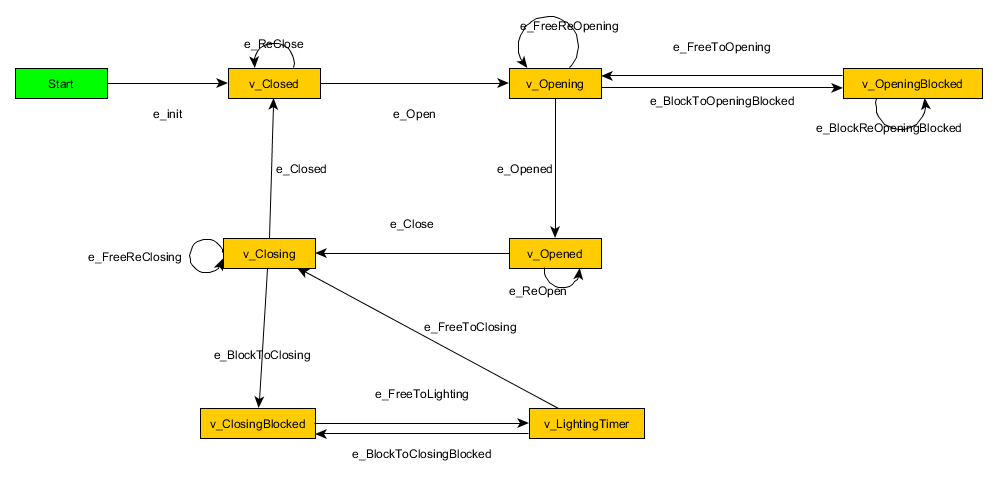
\includegraphics[width=150mm, keepaspectratio]{figures/GateModel.png}
	\caption{Gate Controller model}
	\label{fig:GateModel}
\end{figure}

The control comes to that vertex, which have the some keyword. This model is simple because the lamp can be in a \textit{Lighting} state and can be \textit{Off}.

\begin{figure}[!ht]
	\centering
	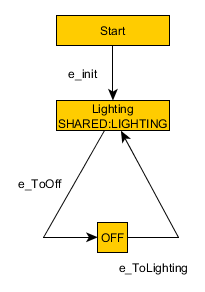
\includegraphics[width=50mm, keepaspectratio]{figures/LightingModel.png}
	\caption{Lamp model}
	\label{fig:LampModel}
\end{figure}

\section{Test adaptation code and test scenario}
For the Gate Controller model I have defined the following test scenarios by the GraphWalker command:
\begin{lstlisting}
@GraphWalker(start = "e_init", value = "random(vertex_coverage(100))")
\end{lstlisting}

The test's goal is to achieve the 100\% vertex coverage by random algorithm, because the software system must be able to function in every possible states.

For each vertex and edge in the model, GraphWalker have generated a method. In the test adaptation phase I have implemented these methods to call the SUT functions, for example:

\begin{lstlisting}
//Create a new instance from the SUT
public GateModelTest() {
	super();
	gate = new GarageGate(); 
}
//implement the e\_Open edge
@Override
public void e\_Open() {
	gate.Open();
}
\end{lstlisting}

\section{Test execution results}
I have run tests on the gateModel with 100\% vertex coverage and as we can see on the next result snippet, the tests reached all vertexes (\textit{"totalNumberOfUnvisitedVertices": 0}).

\begin{lstlisting}
[INFO] Result :
[INFO] {
"totalFailedNumberOfModels": 0,
"totalNotExecutedNumberOfModels": 0,
"totalNumberOfUnvisitedVertices": 0,
"verticesNotVisited": [],
"totalNumberOfModels": 1,
"totalCompletedNumberOfModels": 1,
"totalNumberOfVisitedEdges": 12,
"totalIncompleteNumberOfModels": 0,
"edgesNotVisited": [
{
"modelName": "GateModel",
"edgeId": "e2",
"edgeName": "e_Free"
},
{
"modelName": "GateModel",
"edgeId": "e6",
"edgeName": "e_BlockToClosingBlocked"
},
{
"modelName": "GateModel",
"edgeId": "e7",
"edgeName": "e_FreeToClosing"
}
],
"vertexCoverage": 100,
"totalNumberOfEdges": 15,
"totalNumberOfVisitedVertices": 7,
"edgeCoverage": 80,
"totalNumberOfVertices": 7,
"totalNumberOfUnvisitedEdges": 3
}
\end{lstlisting}

The result also contains information about which edges was not visited: e\_Free, e\_BlockToClosingBlocked, e\_FreeToClosing. To make sure that these are not inaccessible edges I have run a test with 80\% edge\_coverage function.
The result:
\begin{lstlisting}
[INFO] Result :
[INFO] {
"totalFailedNumberOfModels": 0,
"totalNotExecutedNumberOfModels": 0,
"totalNumberOfUnvisitedVertices": 1,
"verticesNotVisited": [{
"modelName": "GateModel",
"vertexName": "OpeningBlocked",
"vertexId": "n7"
}],
"totalNumberOfModels": 1,
"totalCompletedNumberOfModels": 1,
"totalNumberOfVisitedEdges": 12,
"totalIncompleteNumberOfModels": 0,
"edgesNotVisited": [
{
"modelName": "GateModel",
"edgeId": "e11",
"edgeName": "e_BlockToOpeningBlocked"
},
{
"modelName": "GateModel",
"edgeId": "e12",
"edgeName": "e_FreeToOpening"
},
{
"modelName": "GateModel",
"edgeId": "e13",
"edgeName": "e_BlockReOpeningBlocked"
}
],
"vertexCoverage": 85,
"totalNumberOfEdges": 15,
"totalNumberOfVisitedVertices": 6,
"edgeCoverage": 80,
"totalNumberOfVertices": 7,
"totalNumberOfUnvisitedEdges": 3
}
\end{lstlisting}

As we can see from the result there are 3 unvisited edges out of 15, which is 80\% coverage.

\clearpage
%TODO implement PyModel stuff
\section{PyModel implementation}